\documentclass{ctexart}

\usepackage{tikz}
\usetikzlibrary{arrows.meta, trees}
\usetikzlibrary{graphs}

\begin{document}
\section{11.6 结点树}
样式1\\
    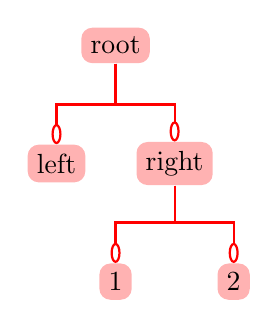
\begin{tikzpicture}
        [edge from parent fork down,
         sibling distance=15mm, 
         level distance=15mm,
         every node/.style={
             fill=red!30,
             rounded corners
         },
         edge from parent/.style={
             red,
             -{Ellipse[open]},
             thick,
             draw
         }
         ]
        \node {root}
        child {node {left}}
        child {node {right}
            child {node {1}}
            child {node {2}}
            };
    \end{tikzpicture}\\
样式2\\
    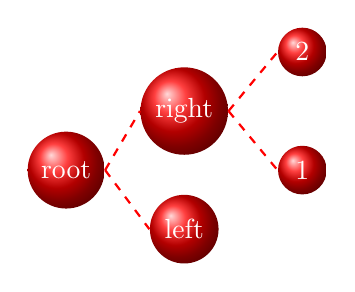
\begin{tikzpicture}
        [
            parent anchor=east,
            child anchor=west,
            grow=east,
            every node/.style={
                ball color=red,
                circle,
                text=white
            },
            edge from parent/.style={
                draw,
                dashed, 
                thick,
                red
            }
         ]
        \node {root}
        child {node {left}}
        child {node {right}
            child {node {1}}
            child {node {2}}
            };
    \end{tikzpicture}

\section{11.7 指定图的句法}
树的延伸方向默认是向右,分支的延伸方向默认是向下。\\
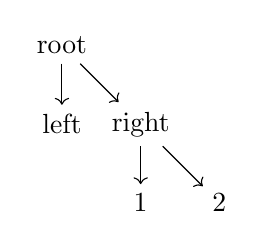
\begin{tikzpicture}
    \graph [grow down, branch right] {
        root -> {left, right -> {1,2}}
    };
\end{tikzpicture}
\tikz \graph [] {
    a -> {b,c,d -> {e,f -> g}}
};

\section{11.8 图形参数的分组}

\hbox{使用scope环境包含相同的图形参数(分组)。}

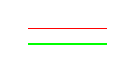
\begin{tikzpicture}
    \begin{scope}[color=red]
        \draw (0,10mm)--(10mm,10mm);
        \draw[green] (0,8mm) -- (10mm,8mm);
    \end{scope}
\end{tikzpicture}

\end{document}